\documentclass{article}
\usepackage{graphicx} % Required for inserting images
\usepackage{hyperref}
\usepackage{amsmath}

\usepackage{caption}
\usepackage{subcaption}

\usepackage{biblatex}
\addbibresource{references.bib}

\graphicspath{ {./figures/} }

\title{Numerical schemes in \textit{CFd-rs}}
\author{
    Xavier N.\\
}
\date{September 2025}
\begin{document}

\maketitle

\section{Gradient}
    
    \subsection{Green-Gauss method}
        
        \subsubsection{Compact stencil}
            
            See~\cite[p.~278]{fvm-basics}.
            
            \[\phi_f = \frac{\phi_C + \phi_F}{2} + \frac{1}{2}((\nabla \phi)_C + (\nabla \phi)_F) \cdot (\mathbf{x}_f - \frac{\mathbf{x}_C + \mathbf{x}_F}{2})\]
            \[(\nabla \phi)_C = \sum_f \phi_f S_f \mathbf{n}_f \]
            
            ~\\
            
            \textbf{Neumann}
                
                $(\nabla \phi)_f \cdot \mathbf{n}_f = q$ is known. 
                
                \[\phi_f = \phi_C + q (\mathbf{x}_f - \mathbf{x}_C) \cdot \mathbf{n}_f\]
    
\section{Laplacian}
    
    \subsection{Orthogonal correction}
        
        \[\mathbf{d}_{CF} = \mathbf{x}_F - \mathbf{x}_C\]
        \[\mathbf{e}_{CF} = \frac{\mathbf{d}_{CF}}{|\mathbf{d}_{CF}|} S_f\]
        \[\mathbf{t}_{CF} = \mathbf{n}_f S_f - \mathbf{e}_{CF}\]
        \[\int_V \nabla \cdot (\nabla \phi) dV = \sum_f ( \underbrace{S_f \frac{\phi_C - \phi_F}{|\mathbf{d}_{CF}|}}_\text{Implicit} + \underbrace{\mathbf{t}_{CF} \cdot \nabla \phi_f}_\text{Explicit} ) \]
    
    
\section{Poisson}
    
    \begin{figure}[ht!]
        \centering
        \begin{subfigure}[b]{1.\textwidth}
            \centering
            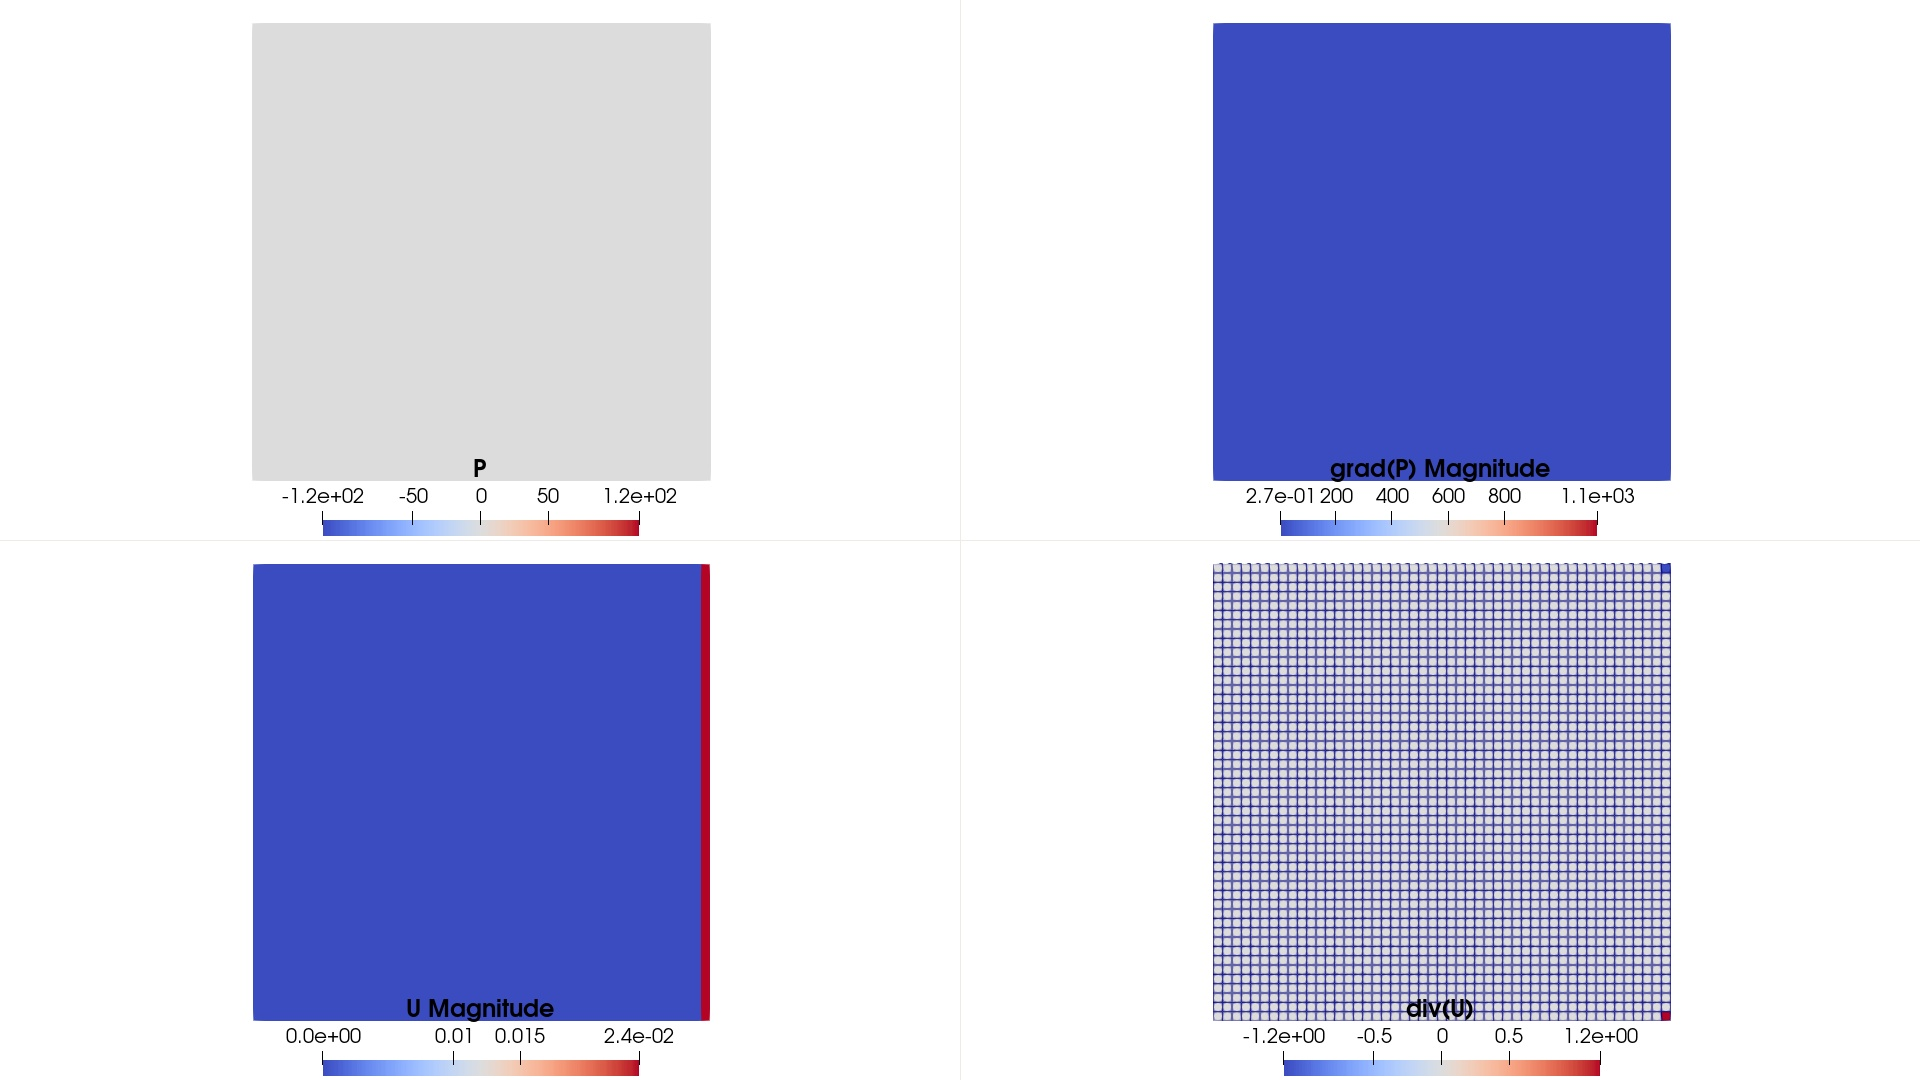
\includegraphics[width=\textwidth]{test-poisson/pred.jpeg}
            \caption{After prediction step}
            \label{fig:pred}
        \end{subfigure}
        \vfill
        \begin{subfigure}[b]{1.\textwidth}
            \centering
            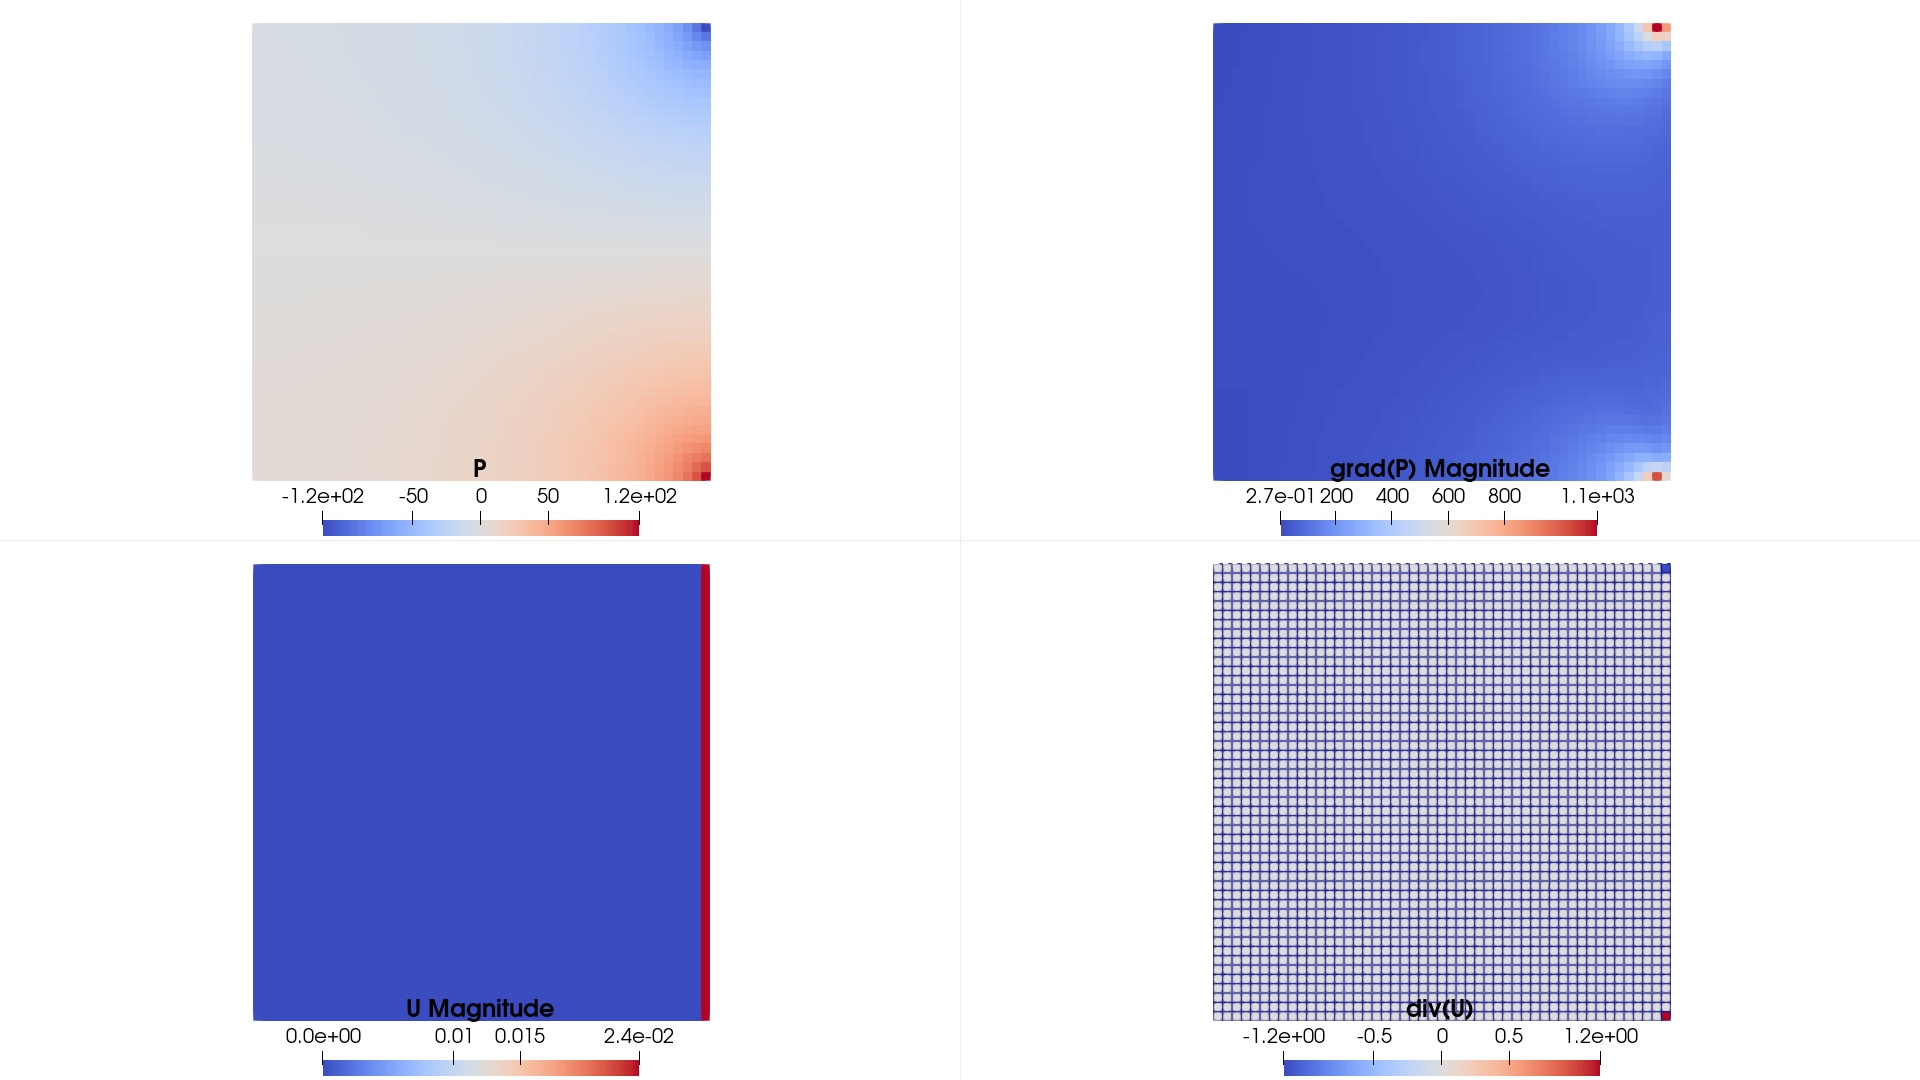
\includegraphics[width=\textwidth]{test-poisson/poisson.jpeg}
            \caption{After pressure computation}
            \label{fig:poisson}
        \end{subfigure}
        \vfill
        \begin{subfigure}[b]{1.\textwidth}
            \centering
            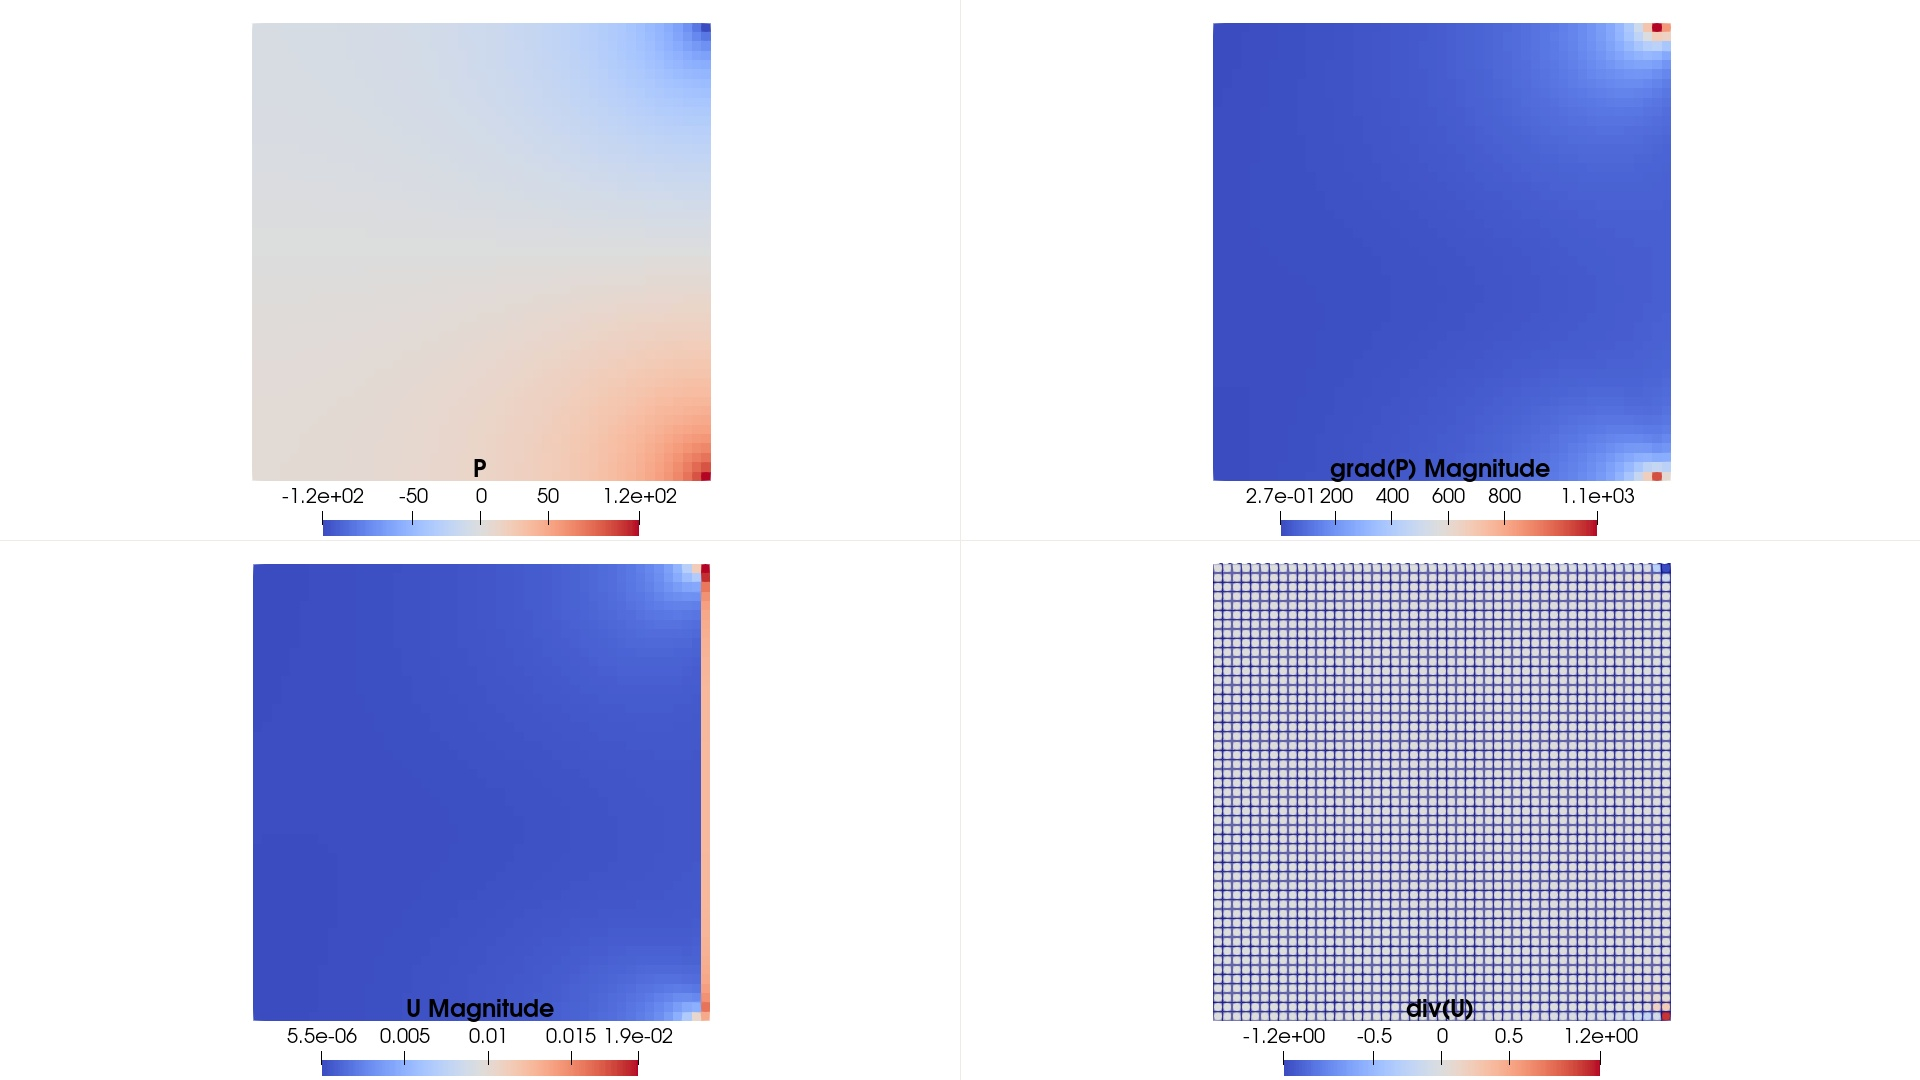
\includegraphics[width=\textwidth]{test-poisson/correction.jpeg}
            \caption{After correction step}
            \label{fig:corr}
        \end{subfigure}
        \caption{Velocity and pressure after different steps of the iteration}
        \label{fig:poisson-test}
    \end{figure}
        
\end{document}